
\documentclass[usenames, dvipsnames, tikz]{standalone}

\usepackage{tikz}
\usetikzlibrary{calc}
\usepackage{ifthen}
\usetikzlibrary{patterns}

\begin{document}


% custom grid spacing from
% http://tex.stackexchange.com/a/119705/4912

\pgfdeclarepatternformonly[\LineSpace]{my north east lines}{\pgfqpoint{-1pt}{-1pt}}{\pgfqpoint{\LineSpace}{\LineSpace}}{\pgfqpoint{\LineSpace}{\LineSpace}}%
{
    \pgfsetlinewidth{1.0pt}
    \pgfpathmoveto{\pgfqpoint{0pt}{0pt}}
    \pgfpathlineto{\pgfqpoint{\LineSpace + 0.1pt}{\LineSpace + 0.1pt}}
    \pgfusepath{stroke}
}

\newdimen\LineSpace
\tikzset{
    line space/.code={\LineSpace=#1},
    line space=6pt
}

% nodes with pattern fill from 
% http://tex.stackexchange.com/a/50945/4912


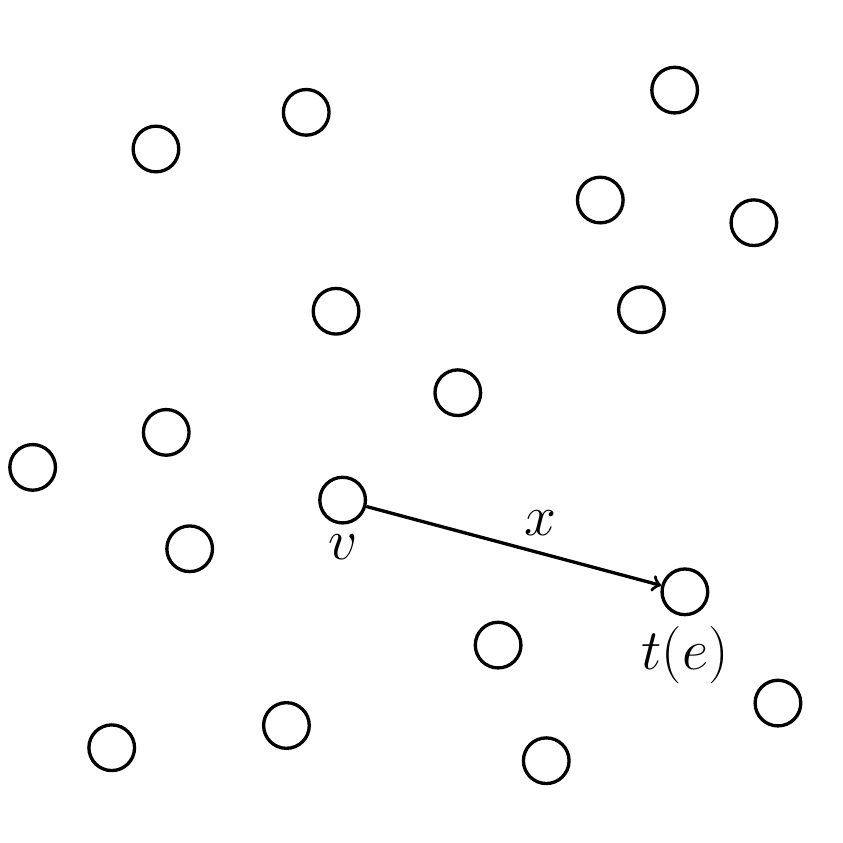
\begin{tikzpicture}[inmargin_node/.style={draw, very thick, circle, inner
                      sep=0, minimum size = 16.5},
                    outmargin_node/.style={draw, circle, very thick, inner
                      sep=0, minimum size = 16.5}]

  \def \Edge {10.}
  \def \Distance {4.5}
  \def \Margin {1.0}

  \pgfmathsetseed{1211995}


  \path[use as bounding box] (0,0) rectangle (\Edge,\Edge);

  \node[outmargin_node, label=below:{\huge$v$}]  (Origin) at (4,4) {};

  \foreach \i in {1,2,..,5}{
    \pgfmathsetmacro{\X}{rnd*\Edge}
    \pgfmathsetmacro{\Y}{rnd*\Edge}


    \pgfmathsetmacro{\XYDist}{((\X-4)^2 + (\Y-4)^2)^(0.5)}
    \pgfmathsetmacro{\InBound}{\Distance-\Margin}
    \pgfmathsetmacro{\OutBound}{\Distance+\Margin}

    %Use \lenghttest with pt values for float comparison, latex can't
    %do it otherwise, see http://stackoverflow.com/a/2782751/692634
    %
    %Syntax: \ifthenelse{<statement>}{<do if true}{<do if false>}

    \ifthenelse{\lengthtest{\InBound pt < \XYDist pt} \AND \lengthtest{\XYDist pt < \OutBound
        pt}}{\node[inmargin_node] at (\X,\Y) {};}{\node[outmargin_node] at
        (\X,\Y) {};} }


  %\node[draw, circle, inner sep=0, minimum size=10, fill=gray!25]
  % (t_1) at (7,4) {};

  \node[inmargin_node] (Target) at
  ($(Origin) +(32.5:\Distance)$) {};

  \node[inmargin_node] (t1) at
  ($(Origin) +(118:\Distance+\Margin*0.55)$) {};

  \node[inmargin_node, label=below:{\huge$t(e)$}] (t2) at
  ($(Origin) +(345:\Distance)$) {};

  \node[outmargin_node] at ($(Origin)+(43:2.0)$) {};
  \node[outmargin_node] at ($(Origin)+(317:2.7)$) {};
  \node[outmargin_node] at ($(Origin)+(256:2.95)$) {};
  \node[outmargin_node] at ($(Origin)+(159:2.4)$) {};
  \node[outmargin_node] at ($(Origin)+(92:2.4)$) {};
  \node[outmargin_node] at ($(Origin)+(51:6.7)$) {};
  \node[outmargin_node] at ($(Origin)+(34:6.3)$) {};
  \node[outmargin_node] at ($(Origin)+(335:6.1)$) {};

  \node[inmargin_node] at ($(Origin)+(308:\Distance+\Margin*-0.3)$) {};
  \node[inmargin_node] (et) at ($(Origin)+(227:\Distance+\Margin*-0.2)$) {};


  
  % \draw[dashed, thick] (Origin) circle (\Distance+\Margin);
  % \draw[dashed, thick] (Origin) circle (\Distance-\Margin);


  % --------- Original ------- $

  \draw[very thick, ->] (Origin) -- node[auto]{\huge $x$} (t2);
  % \draw[very thick, ->, gray] (Origin) -- (et);

  % \node[label=above:{\huge2$\varepsilon$}] (width_center) at ($(Origin)+(0:\Distance)$) {}; 
  % \draw[dashed, domain=348:360] plot ({4+\Distance*cos(\x)},{4+\Distance*sin(\x)}); 

  % \draw[very thick, <-] ($(Origin)+(\Distance-\Margin,0)$) --   (width_center);
  % \draw[very thick, ->] (width_center)--
  % ($(Origin)+(\Distance+\Margin,0)$);


  % --------- Rewired  ------- $

  % \draw[very thick, ->] (Origin) -- (t1);


\end{tikzpicture}
\end{document}
%%% Local Variables: 
%%% mode: latex
%%% TeX-master: t
%%% End: 
